\chapter{Lecture 11 Sparse Matrices and Iterative Solution Methods}
\label{ch:lec11n}
\section{Objectives}
The objectives of this lecture are to:
\begin{itemize}
\item Describe sparse matrices and their importance in scientific computing.
\item Introduce some interative solution methods.
\item Show some examples.
\end{itemize}
\setcounter{lstannotation}{0}

\section{Introduction}
Up to this point we have discussed a handful of methods for solving linear systems of equations.  We studied Gauss elimination with and without pivoting; LU factorization which, to be sure, is basically the same as Gauss elimination.  We also learned a little bit about the array of solution methods that are used in MATLAB's built-in tools for linear equations.  These are fundamental methods that should be in the toolbox of every engineer.

There are pratical situations where these direct solution methods for linear equations are not suitable.  Physical conservation laws that are encoded in partial differential equations, discretized and solved using methods like the finite element method (FEM) and finite volume method (FVM) results in large systems of linear equations.  A high-resolution simulation will routinely require upwards of $10^5$ degrees of freedom\sidenote{In this context, the number of \emph{degrees of freedom} can be interpreted to refer to the length of a vector describing the unknown function.} to adequately resolve the physics of interest such as: the flow field around an automobile to estimate drag forces; stress and strain distribution within a complex structural component to ensure material failure limits are not exceeded; or the component temperature in the vicinity of a weld process.

Just \emph{storing} the matrices used to represent these linear systems---something, for example, like a $10^5 \times 10^5$ matrix\sidenote{Such a matrix has $10^{10}$ entries.  If each entry is represented with a double-precision floating point number (8 bytes each), that adds up to roughly 80 Gigabytes of memory just to \emph{store} the matrix.}---requires us to take a new approach from what we have described up to now.  Likewise ``solving'' the systems to find the unknown vectors---whether the vector represents temperature, pressure, a velocity component, or a component of material displacement---requires new techniques.

\section{Sparse Matrices}

Matrices that arise as part of a finite difference method or finite element method is almost always \emph{sparse}.  This means that for every row of the matrix, corresponding to a linear equation pertaining to a single degree of freedom, most of the entries are equal to zero.  

\begin{marginfigure}[-4.0cm]
%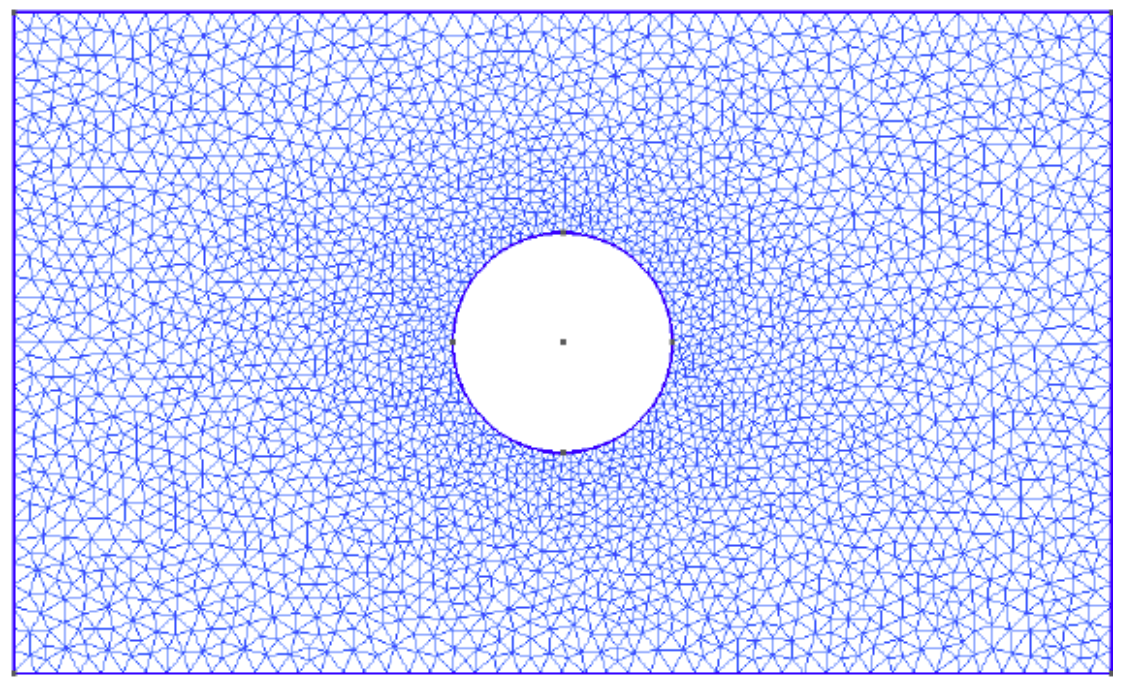
\includegraphics{lec11n-mesh.png}
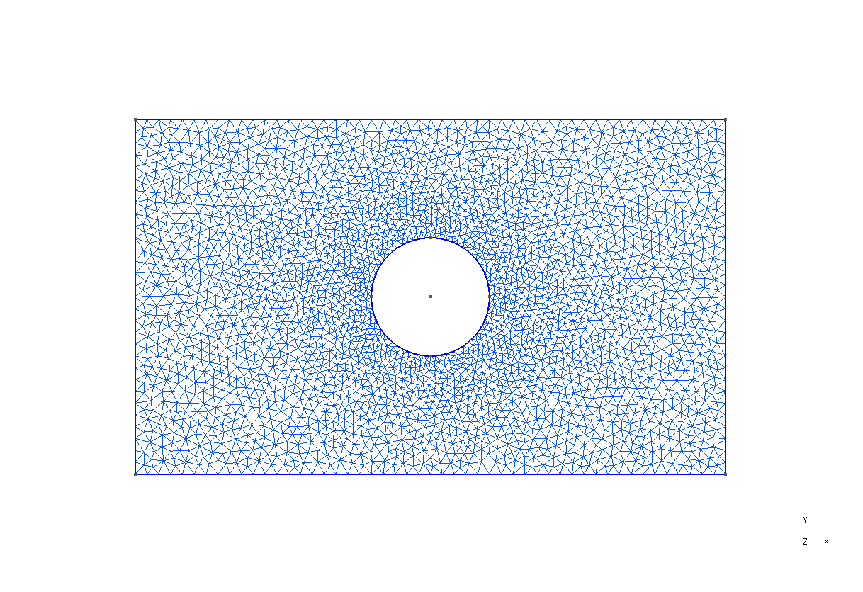
\includegraphics{discretization.eps}
\caption{A triangular mesh for a finite element method analysis of the transient heat equation.}
\label{fig:lec11n-mesh}
\end{marginfigure}
As an example, consider a finite element discretization of the transient heat equation on a domain that is rectangular in shape, but with a hole in the middle.  The mesh is depicted in Figure \ref{fig:lec11n-mesh}. The governing equation is shown in Equation \ref{eq:lec11n-transient-heat}:
\begin{equation}
\frac{k}{\rho c_p}\frac{\partial u}{\partial t} = \nabla^2 u + S
\label{eq:lec11n-transient-heat}
\end{equation}
where $k$ is the thermal conductivity, $\rho$ is density, $c_p$ is the specific heat, $S$ corresponds to a constant uniform heat source, $u$ is the temperature, and $t$ is time. In the finite element method, this equation and specified boundary conditions are translated into a linear system of equations:
\begin{equation*}
Au = b
\end{equation*} 
\begin{marginfigure}[-6.0cm]
%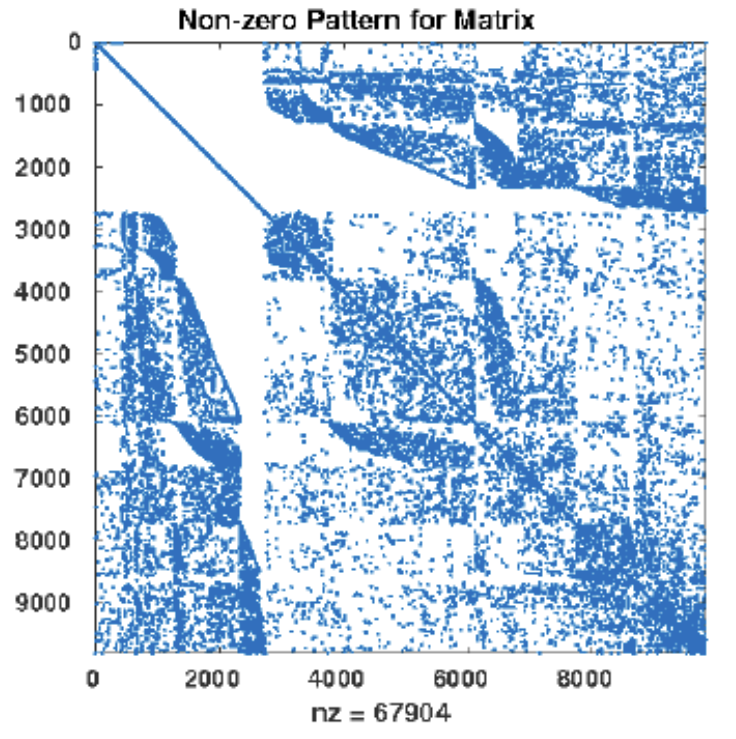
\includegraphics{lec11n-spy1.png}
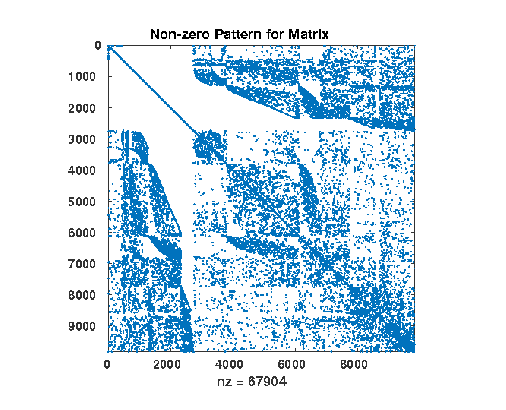
\includegraphics{Thermal_9824.eps}
\caption{Non-zeros in linear system for transient heat conduction.}
\label{fig:lec11n-spy1}
\end{marginfigure}
The non-zero structure of this system of equations can be observed using MATLAB's built-in function \lstinline[style=myMatlab]{spy(A)}, and the result is shown in Figure \ref{fig:lec11n-spy1}. The system of equations has 9824 nodes, each with a single degree of freedom.  The resulting $9824 \times 9824$ matrix $A$ has a total of 67,904 non-zero entries; an average of about 8 non-zero elements per equation.\sidenote[][-3.0cm]{Bottom Line Up Front: this number of non-zeros per row is typical for two-dimensional systems with linear, triangular elements.  The number of non-zeros per equation for the FEM or FVM depends on a number of factors: a) number of degrees of freedom per node; b) the number of spatial dimensions; c) the number of internal degrees of freedom for each finite element among others.  This will be discussed in detail in later lectures on finite element methods.  } This pattern, which is typical for such matrices, can be exploited by only storing and carrying out arithmetic with the non-zero entries of the matrix.  

There are a number of sparse-matrix storage formats in use.  MATLAB uses the compressed-sparse-column (CSC) storage format.\cite{gilbert1992sparse}  If there are $nnz$ non-zero entries in a $n \times n$ sparse array, MATLAB stores one (double precision) vector of length $nnz$ with the non-zero values---call this vector: \lstinline[style=myMatlab]{ENTRY}; another vector of integers of length $nnz$---call this vector: \lstinline[style=myMatlab]{ROW}---with the row-number for each non-zero; and a third vector of integers of length $n+1$---call this vector: \lstinline[style=myMatlab]{COL}---that stores the index (from the \lstinline[style=myMatlab]{ENTRY} array) of the first non-zero from each column.  An example of this format is shown in Figure \ref{fig:lec11n-csc}.  
\begin{marginfigure}
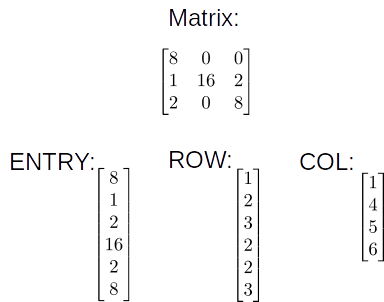
\includegraphics{CSC-example.png}
\caption{Example sparse matrix in Compressed Sparse Column format.}
\label{fig:lec11n-csc}
\end{marginfigure} 
\noindent The total storage required is $nnz \times 8$ bytes for the \lstinline[style=myMatlab]{ENTRY} array + $nnz \times 4$ bytes for the \lstinline[style=myMatlab]{ROW} array + $(n+1) \times 4$ bytes for the \lstinline[style=myMatlab]{COL} array.  In asymptotic notation, $\mathcal{O}(nnz+n)$ bytes of storage are required.  Contrast this with $\mathcal{O}(n^2)$ for dense matrices.  If $nnz << n$ the savings with sparse matrices is huge.  The key issues to keep in mind are these:\marginnote{In terms of FLOPs, sparse matrix calculations are slower.  Dense matrix algorithms are heavily optimized to make best use of the memory heirarchy of common CPUs resulting in high computational intensity and performance.  Sparse matrix algorithms have lower computational intensity and the memory access patterns are harder to optimize for multi-threaded execution.  As a result, sparse matrix operations are relatively slow.  Readers are encouraged to experiment with MATLAB to get a better feel for the relative performance of dense and sparse matrix operations.}
\begin{enumerate}
\item Exploiting the sparsity of these matrices is not a performance enhancement, it is a necessity.  Simulations of practical interest often result in systems of equations that can \emph{only} be stored as a sparse matrix.
\item The resulting matrix, if it is to be solved, \emph{cannot} be solved by Gauss elimination or LU factorization.
\end{enumerate}

The reason for the second point is that, even for matrices that are sparse, the LU-factorization for that matrix usually is not sparse.  The forward elimination process common to both of the aformentioned techniques systematically destroys the sparsity pattern.  This effect is shown in Figure \ref{fig:lec11n-LandU}.
\begin{figure}[h!]
\subfloat[]{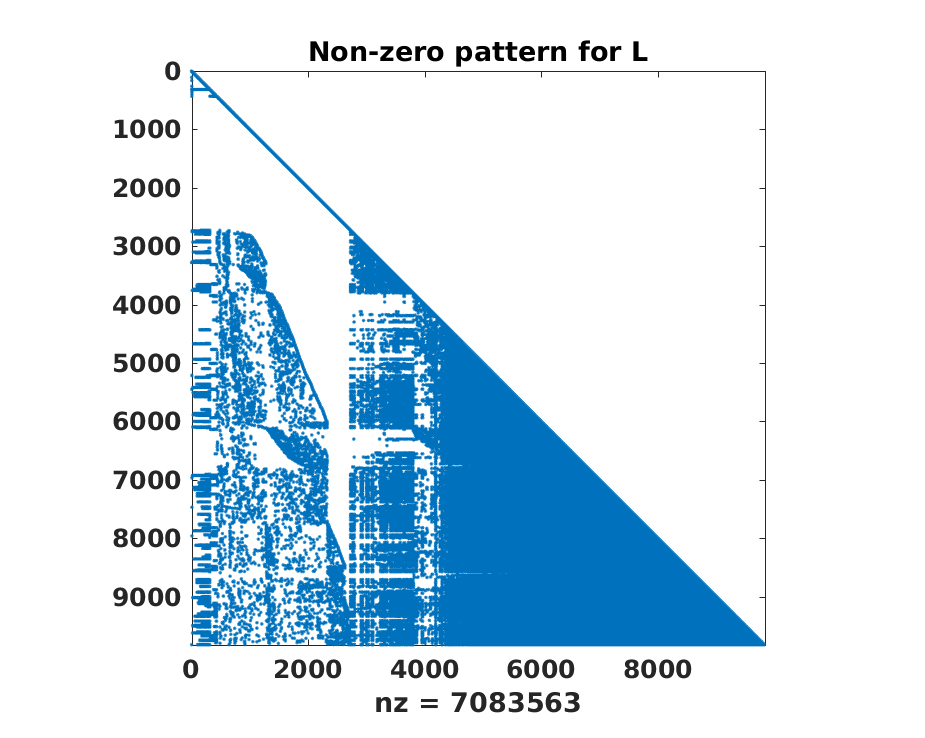
\includegraphics[width=2in]{Non_zero_L_thermal.eps}}
\subfloat[]{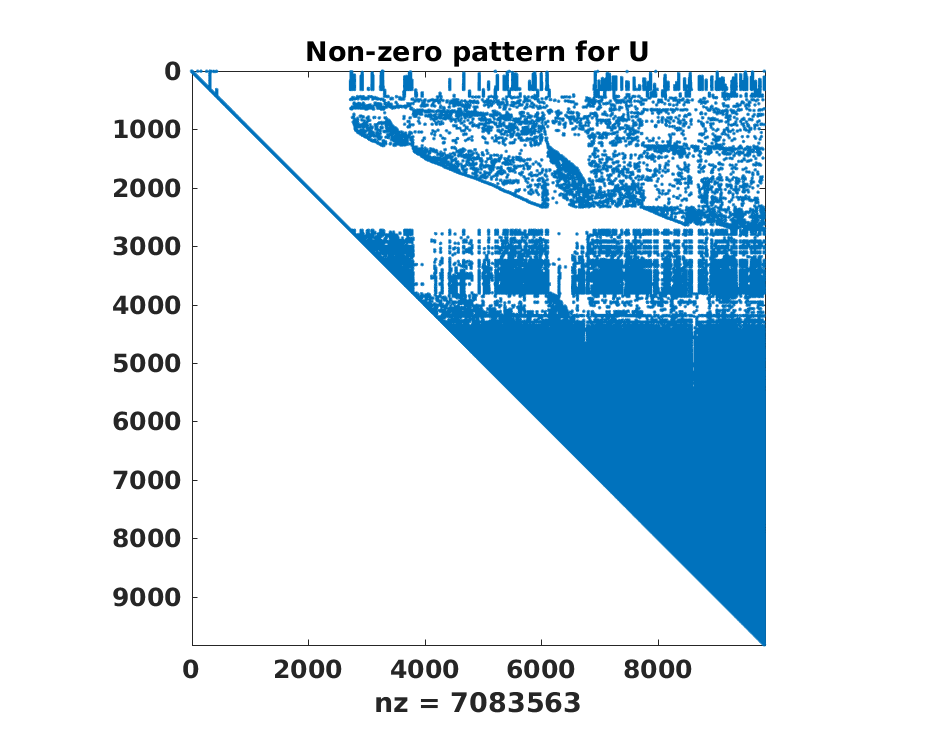
\includegraphics[width=2in]{Non_zero_U_thermal.eps}}
\label{fig:lec11n-LandU}
\caption[][3.0cm]{Sparsity pattern of L and U matrices from decomposition of A.}
\end{figure}

\noindent For the larger systems of equations that we want to solve for more interesting problems, this kind of fill-in is unacceptable.

\section{Iterative Solution Methods}

The fundamental idea of iterative methods for solving linear systems of equations is this: given an initial estimate of the solution, $x_0$, find a method to generate a sequence $x_m$ that is easy to compute and that converges to the solution of $Ax=b$.  The methods that we will discuss in this lecture all involve \emph{splitting} the matrix $A$ into a decomposition $A=M-K$ with $M$ non-singular and very easy to invert.  If this is done, the iterative scheme is as follows:
\begin{align*}
Ax &= b \\
(M-K)x &= b \\
\rightarrow Mx &= Kx + b \\
\rightarrow x &= M^{-1}(Kx + b) \\
&= \underbrace{M^{-1}K}_{R}x + \underbrace{M^{-1}b}_{c}
\end{align*}
The resulting iterative method is shown in Equation \ref{eq:lec11n-iterative-gen}:
\begin{equation}
x^{(k+1)} = Rx^{k} + c
\label{eq:lec11n-iterative-gen}
\end{equation}
where $k$ is the iteration number.

Instead of solving a system of equations by factoring the coefficient matrix, we create what we hope to be a convergent sequence of approximations to the solution by repeated matrix-vector multiplication.  Each matrix-vector multiplication operation takes, for dense matrices, $\mathcal{O}(n^2)$ operations.  Since the matrix $R$ is sparse and operations with zero entries of the matrix are eliminated, each matrix-vector multiplication takes only $\mathcal{O}(n)$ operations.

\subsection{Jacobi Iteration}


